\documentclass[titlepage,landscape]{seminar}
\usepackage{url}
\usepackage{graphicx}
\usepackage{hyperref}
\usepackage{epstopdf}
\usepackage{slides}

\newcommand{\frack}{\frac{1}{k}}
\newcommand{\quarter}{\frac{1}{4}}

\begin{document}

\myslide{
  \heading{Revising the neutral theory}

  \begin{itemize}

  \item Most non-synonymous substitutions are deleterious.

  \item Most molecular variability found in natural populations is
    selectively neutral.

  \item Natural selection is primarily purifying (at the level of
    nucelotide sequences).

  \item Alleles enhancing fitness are rapidly incorporated. Those
    reducing fitness are rapidly eliminated.

  \end{itemize}
}

\myslide{
  \heading{ADH in {\it Drosophila melanogaster}}

  Kreitman (1983) cloned and sequenced 11 alleles at the ADH locus in
  {\it Drosophila melanogaster}

  \begin{itemize}

  \item 2.4kb, 765bp (coding)

  \item 6 distinct sequences, differed from one another at 1-13 sites

  \item Expect: 9-10 amino acid differences

  \item Observed: Only one

  \end{itemize}
  
}

\myslide{
\heading{Kreitman and Aquad\'e} \\
{\small
If mutations are neutral:

\begin{itemize}

\item The substitution rate equals the mutation rate.

\item Diversity within populations will be $\frac{4N_e\mu}{4N_e\mu + 1}$

\item Therefore, the amount of divergence between two species should
  be related to the amount of diversity within each.

\end{itemize}
}

}

\myslide{
\heading{Kreitman and Aquad\'e} \\
{\small
If mutations are neutral:

\begin{itemize}

\item The substitution rate equals the mutation rate.

\item Diversity within populations will be $\frac{4N_e\mu}{4N_e\mu + 1}$

\item Therefore, the amount of divergence between two species should
  be related to the amount of diversity within each.

\end{itemize}

Example: The {\it ADH\/} locus in {\it Drosophila melanogaster\/} and
{\it D. simulans}

\begin{itemize}

\item Calculate the number of ``site equivalents'' in each region of
  the locus.

\item Calculate the number of polymorphic site equivalents

\[
\frac{25}{414+411+129} \approx 0.026
\]

\item Calculate the expected number of polymorphic sites within a
  region assuming the same fraction of polymorphic sites in each
  region. 

\end{itemize}
}
}

\myslide{
\heading{Kreitman and Aguad\'e}

{\small
\begin{center}
\begin{tabular}{l|ccc}
\hline\hline
         & 5' flanking & {\it Adh\/} locus & 3' flanking \\
\hline
Diversity$^1$ \\
\quad Observed & 9     & \color{red}{\bf 14}   & 2    \\
\quad Expected & 10.8  & 10.8 & 3.4  \\
Divergence$^2$ \\
\quad Observed & 86    & 48   & 31   \\
\quad Expected & 55    & \color{red}{\bf 76.9} & 33.1 \\
\hline
\multicolumn{4}{l}{$^1$Number of polymorphic sites within {\it
         D. melanogaster\/}} \\
\multicolumn{4}{l}{$^2$Number of nucleotide differences between {\it
         D. melanogaster\/} and {\it D. simulans}}
\end{tabular}
\end{center}
}

}

\myslide{
\heading{Kreitman and Hudson}

\begin{center}
\resizebox{\textwidth}{!}{\includegraphics{kreitman-hudson.eps}}
\end{center}

}

\myslide{
  \heading{Selection in the human genome}

  \begin{itemize}

  \item HapMap Project: SNPs at ca. 3.2M loci

  \item Four geographic populations:

    \begin{itemize}

      \item Yoruba (Ibadan, Nigeria)
      
      \item Japanese (Tokyo, Japan)

      \item Han Chinese (Beijing, China)

      \item ancestry from northern and western Europe (Utah, USA)
        
    \end{itemize}

  \end{itemize}
}

\myslide{
\heading{$F_{ST}$ outliers}

\begin{center}
\resizebox{\textwidth}{!}{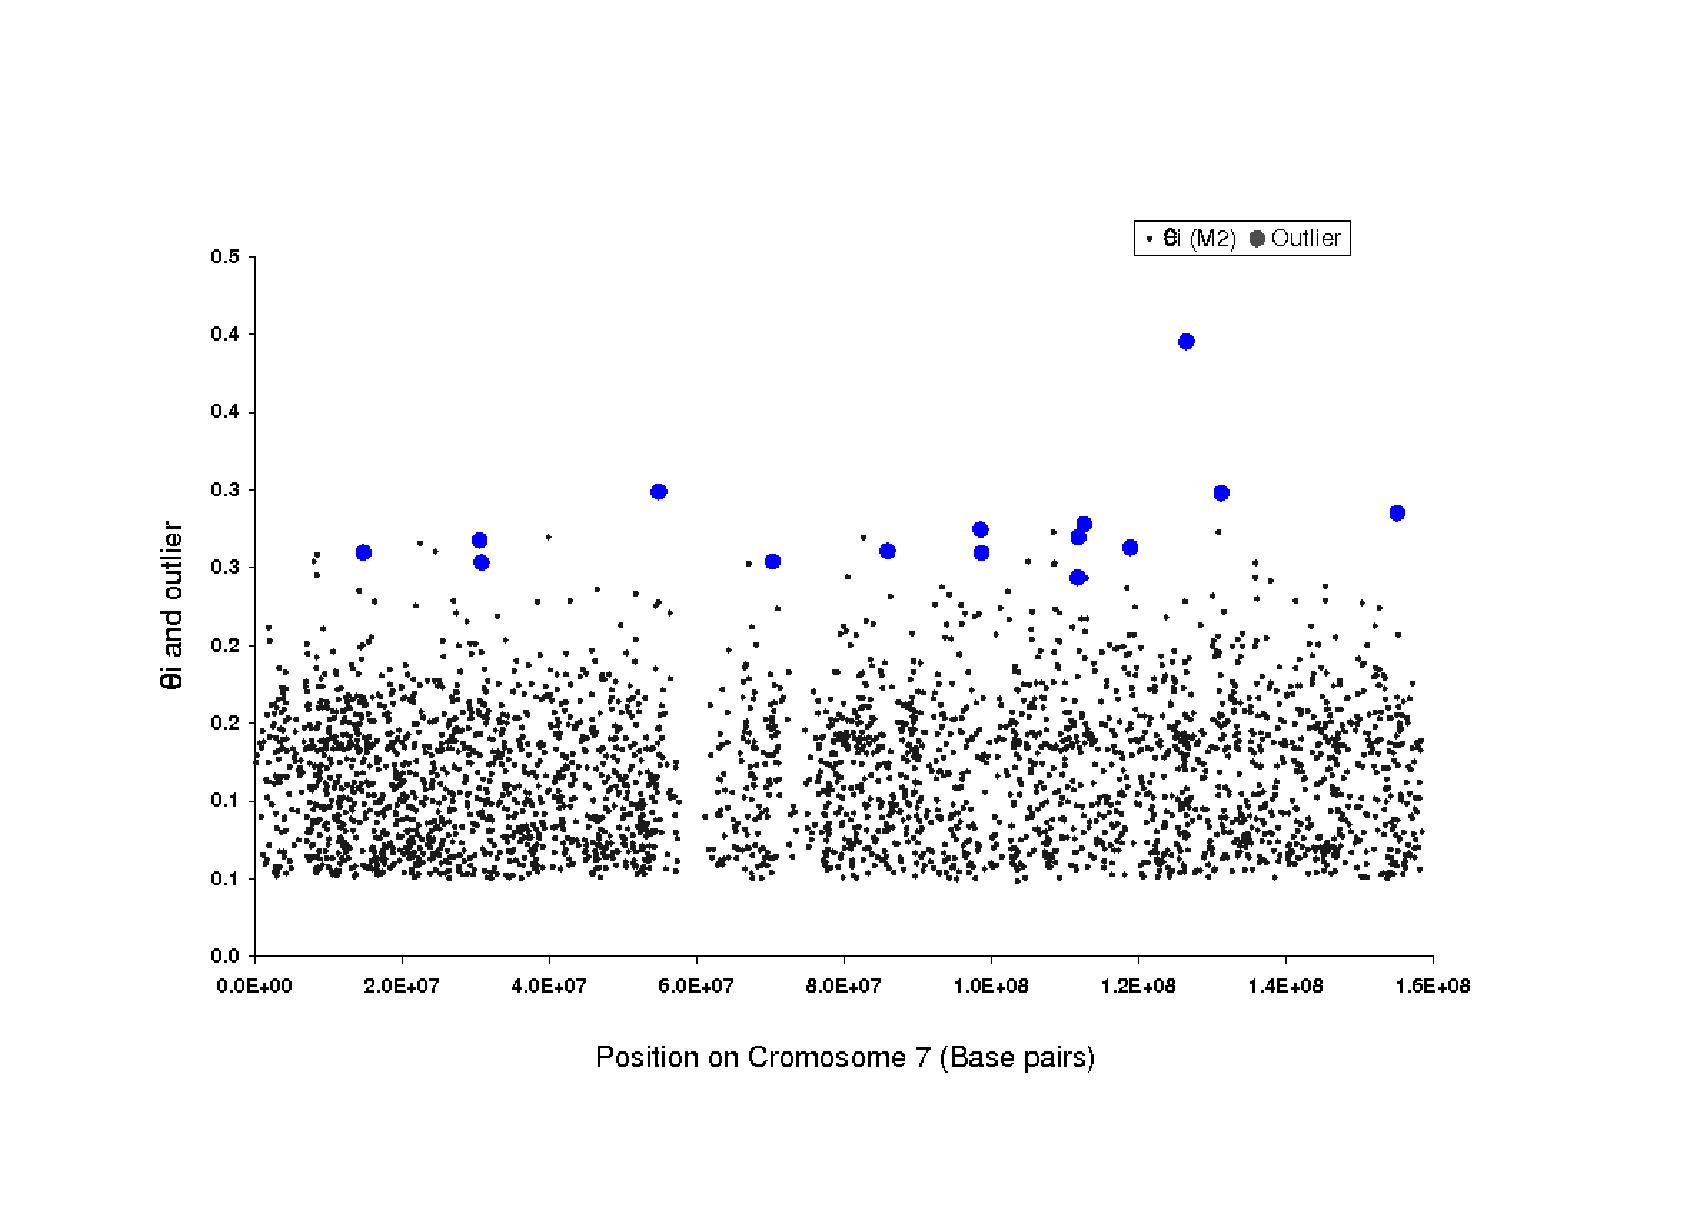
\includegraphics{outlier.eps}}
\end{center}

}

\myslide{
\heading{$F_{ST}$ outliers}

\begin{center}
\resizebox{0.9\textwidth}{!}{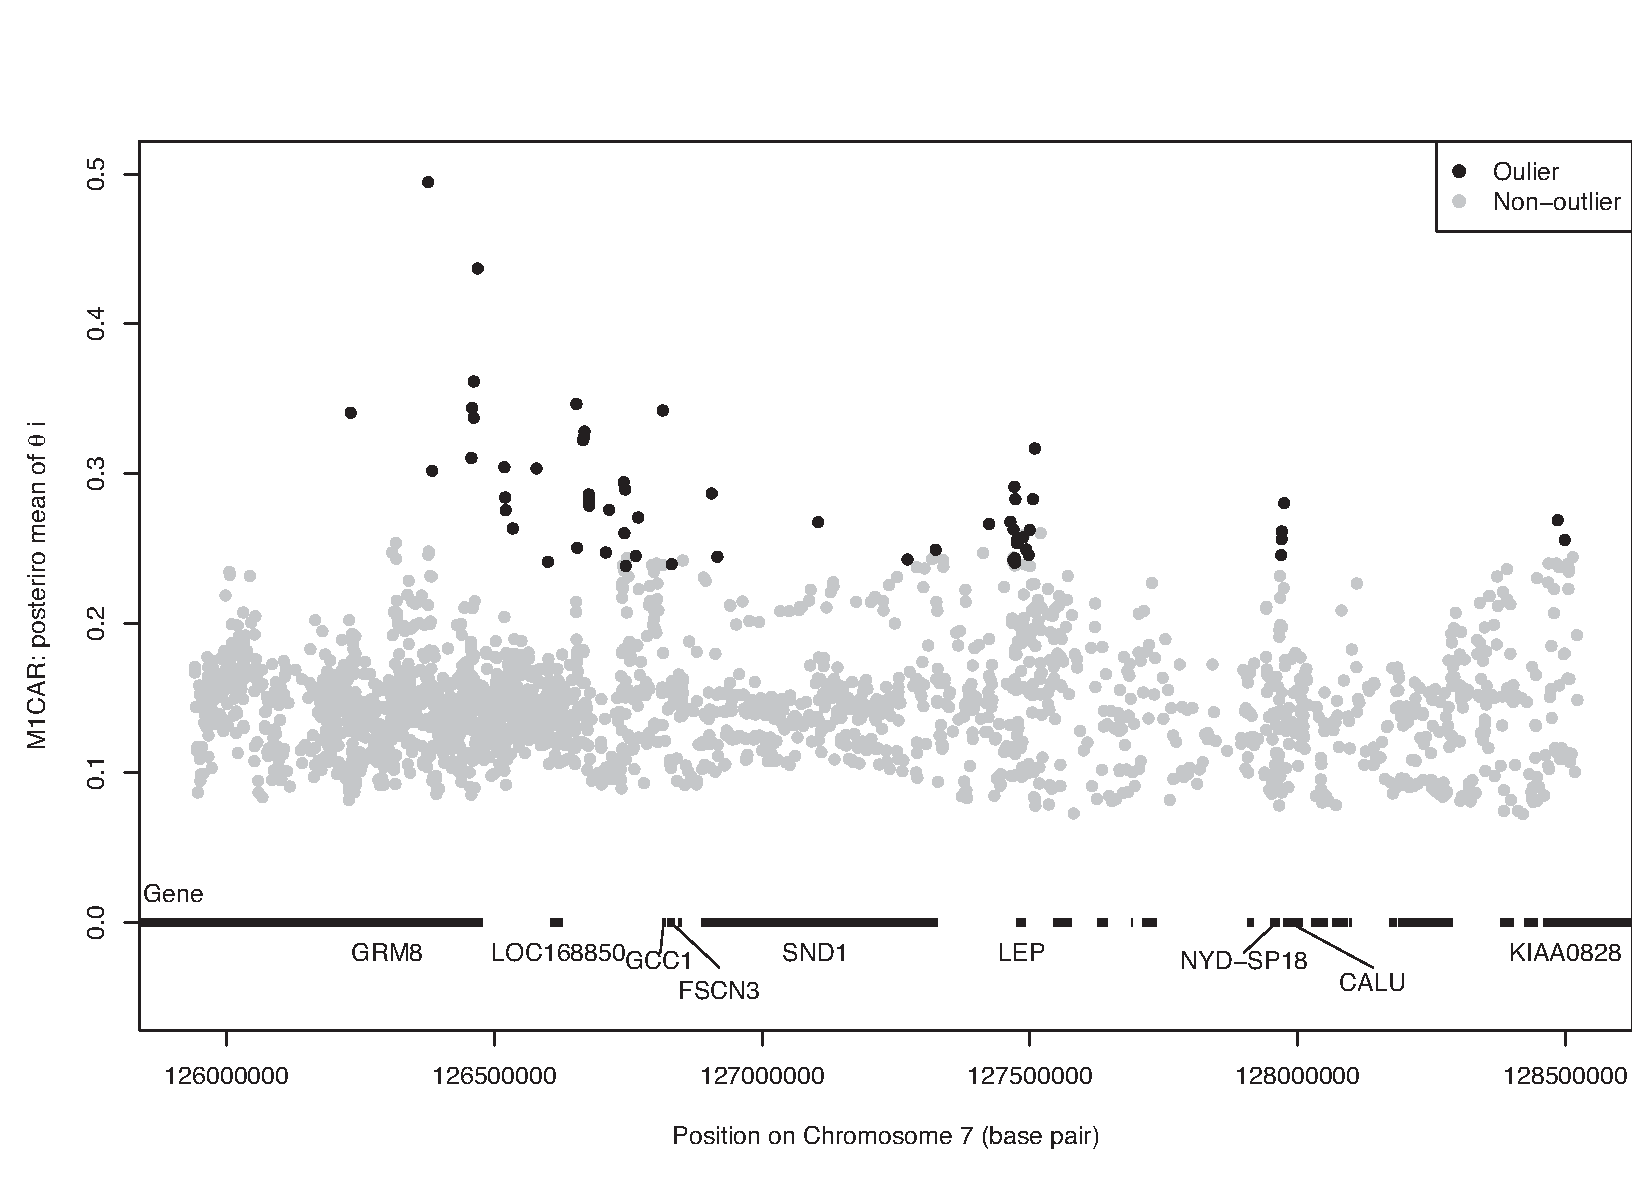
\includegraphics[angle=270]{outlier-high.eps}}
\end{center}

}

\myslide{
\heading{Segregating sites and nucleotide diversity}

\begin{eqnarray*}
k &=& \mbox{number of segregating sites} \\
\hat \pi &=& \sum x_ix_j\delta_{ij}/N ,
\end{eqnarray*}
where $x_i$ is the frequency of haplotype $i$, $\delta_{ij}$ is the
number of nucleotide differences between $i$ and $j$, and $N$ is the
sequence length.
}

\myslide{
\heading{Tajima's $D$}

Let $\theta = 4N_e\mu$. {\bf NOTE}: This is not the same $\theta$ we
encountered when we were doing $F$-statistics.

\begin{eqnarray*}
\mbox{E}(k) &=& \theta \sum_i^{n-1} \frac{1}{i} \\
\mbox{E}(\pi) &=& \theta
\end{eqnarray*}

Two estimates of $\theta$:

\begin{eqnarray*}
\hat\theta_{\pi} &=& \hat \pi \\
\hat\theta_k &=& \frac{k}{\sum_i^{n-1} \frac{1}{i}}
\end{eqnarray*}
}

\myslide{
\heading{Tajima's $D$}

\[
\hat D = \theta_{\pi} - \theta_k
\]

\begin{description}

\item[Neutral variation] $\hat D \approx 0$ 

\item[Overdominant selection] $\hat D > 0$

\item[Population bottleneck] $\hat D > 0$

\item[Purifying selection] $\hat D < 0$

\item[Population expansion] $\hat D < 0$

\end{description}

}

\myslide{
\heading{Nucleotide diversity}

\begin{eqnarray*}
\pi &=& \sum_{ij} x_ix_j \delta_{ij} \\
x_i &=& \mbox{frequency of haplotype $i$} \\
\delta_{ij} &=& \mbox{fraction of nucleotides at which $i$ and $j$ differ}
\end{eqnarray*}

Now suppose we have samples from different populations.

\[
x_{ik} = \mbox{frequency of haplotype $i$ in population $k$}
\]

}

\myslide{
\heading{Analysis of Molecular Variance (AMOVA)}

Mean frequency of haplotype $i$:
\[
x_{i\cdot} = \frac{1}{K}\sum_{k=1}^K x_{ik}
\]

\vfill

Nucleotide diversity within the whole sample and within populations:
\begin{eqnarray*}
\pi_t &=& \sum_{ij} x_{i\cdot}x_{j\cdot} \delta_{ij} \\
\pi_s &=& \frac{1}{K}\sum_{k=1}^K\sum_{ij} x_{ik}x_{jk}\delta_{ij}
\end{eqnarray*}

}

\myslide{
\heading{Analysis of Molecular Variance (AMOVA)}

\[
\Phi_{st} = \frac{\pi_t - \pi_s}{\pi_t}
\]

\vfill

A trip down memory lane
\[
F_{ST} = \frac{H_t - H_s}{H_t} 
\label{eq:f-st}
\]
}

\myslide{
\heading{Differences to distances}
\begin{center}
\resizebox{!}{0.9\textheight}{\includegraphics{amova-procedure.eps}}
\end{center}
}

\myslide{
\begin{center}
\resizebox{!}{0.9\textheight}{\includegraphics{amova-sample-locations.eps}}
\end{center}
}

\myslide{
\begin{center}
\resizebox{!}{0.9\textheight}{\includegraphics{amova-haplotypes.eps}}
\end{center}
}

\myslide{
\heading{AMOVA results}

\begin{center}
\begin{tabular}{lc}
\hline\hline
Component of differentiation     & $\Phi$-statistics \\
\hline
Among regions                    & $\Phi_{CT} = 0.220$ \\
Among populations within regions & $\Phi_{SC} = 0.044$ \\
Among all populations            & $\Phi_{ST} = 0.246$ \\
\hline
\end{tabular}
\end{center}

\vfill

\begin{eqnarray*}
1 - \Phi_{ST} &=& (1 - \Phi_{SC})(1 - \Phi_{CT}) \\
0.754 &=& (0.956)(0.78)
\end{eqnarray*}

}

\myslide{
\heading{Ancestral polymorphism}

\begin{center}
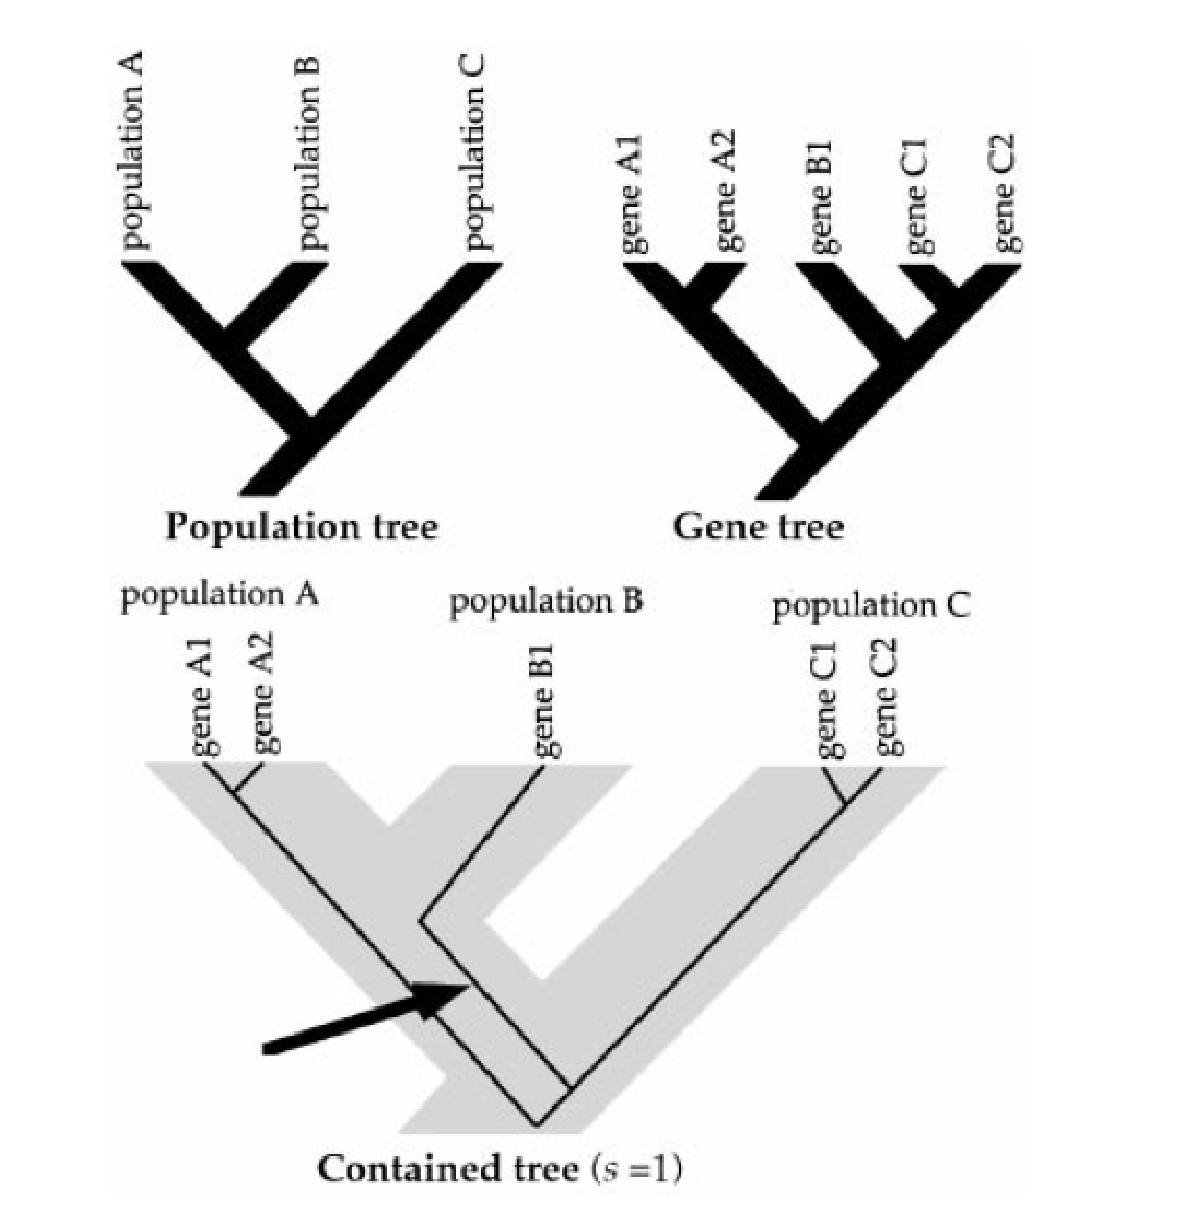
\includegraphics[height=0.9\textheight]{ancestral-polymorphism.eps}
\end{center}

}

\myslide{
\heading{The coalescent in structured populations}

Remember that in a single population
\[
P(t|k, N_e) = \left(\frac{k(k-1)}{4N_e}\right)\left(1-
  \frac{k(k-1)}{4N_e}\right)^{t-1}
\]

\begin{eqnarray*}
P_k(\mbox{coalescent}|n, N_e) &=& \frac{k(k-1)}{4N_e} \\
P(\mbox{no coalescent}|k, N_e, K)
                              &=&\left(1-\frac{k(k-1)}{4N_e}\right)^K \\
P(\mbox{no migration}|k,m, K) &=& (1-m)^{kK}
\end{eqnarray*}
}

\myslide{
\heading{The coalescent in structured populations}


{\scriptsize
\begin{eqnarray*}
P(\mbox{event}|k, m, N_e, K) &=& 1 - P(\mbox{no coalescent}|k, N_e,
K)P(\mbox{no migration}|k,m, K)
\end{eqnarray*}
}

{\small
\[
P(\mbox{event at }t|k, m, N_e, K) = P(\mbox{event}|k, m, N_e,
K)\left(1 - P(\mbox{event}|k, m, N_e, K)\right)^{t-1} 
\]

\[
P(\mbox{data}|m, N_e) \propto f(n, m, N_e, K)
\]

}

}

\myslide{
  \heading{How much genetic change is due to selection?}

  \begin{itemize}

    \item Estimate allele frequencies at many loci at several
      different time steps.

    \item Define $\Delta p_t = p_{t+1} - p_t$.

    \item Let $\mbox{Var}(\Delta p_t)$ be the variance of $\Delta p_t$
      across loci.

    \item Buffalo and Coop (2019) point out that

      \[
        \mbox{Var}(\Delta p_t) = \sum_{i=0}^{i-1}\mbox{Var}(\Delta
        p_i) + \sum_{i \ne j} \mbox{Cov}(p_i, p_j)
      \]

    \item The covariance is due to selection causing correlated
      changes in allele frequency at different loci.

  \end{itemize}
}

\myslide{
  \heading{How much genetic change is due to selection?}

  \begin{itemize}

  \item Selection for high temperature tolerance

  \item 10 replicate populations, 10 generations

  \item Between 17 and 37 percent of allele frequency changes are a
    result of natural selection.

  \end{itemize}
}

\end{document}
